


\subsection{Changes in design and implementation (Roar)}
%What was changed compared to design section? (short list)

At first, the program was comprised of the classes: BankApplication, User, Account and an auxiliary class called Database. These were implemented as the core of the program, with the User and Account as the model and BankApplication as the controller, deciding what changed needs to be done to the model. The Database class' only purpose was to simulate the interaction with the database. All methods in the Database class gave an overview of which statemets needed to be executed, when implementing the actual database connection. No UI was created at this point, since the application was tested with direct method calls. 

The next big step was to divide the users into customers and admins. The User class was made abstract and is extended by the Customer and Admin classes. This made it possible to distinguish between customers and admins when features were allowed to one, but not the other.

Then the application was made to run on a java servlet, turning the application into a web application. The servlet was implemented in the DefaultServer class, and was the main link between the user and the application. This way the application has two main control classes, being the DefaultServer and the BankApplication with each their task. The DefaultServer acts upon input from the UI's, deciding what has to be changed in the model. The DefaultServer informs the BankApplication which changes are to be executed. The BankApplication commits the changes in the model, and provides the DefaultServer with any requested information. The DefaultServer collects the information needed to setup the UI for the user.

When the database connection was implemented, the Database class was substituted with a class called DatabaseProtocol. This class contained the same features as the Database class, but instead of local storage in arrays, the data was stored in the DALLASB database delivered by IBM. Once the database was connected, the design of the program, was as planned, and has changed very little during the subsequent sessions. 

Besides the mentioned classes, some UI classes and exception classes were created. The exception classes help control the dataflow, when unwanted behavior was encountered, as mentioned in the Security section. The UI classes, comprised of .html and .jsp files, deliver the user input to the server in the form of HTML forms.

\subsection{Implementation decisions (Roar)}

During the evolution of the application described in the section above, some decisions were made:

Implementing the core of the program locally and testing it without the need of any web connections, was chosen for several reasons. The tools needed to connect the the program with e.g. the database was not granted from the start of the course. Implementing the program locally made it possible to brainstorm and test how the program should work early, instead of waiting for the necessary tools to be available. Testing features is also kept simple, when a preset data is set each time the program is run, which is fast and easy when it is not using a remote database. 

Choosing to devide users into customers and admins, was a good way to get an overview of the different accounts without looking in the database directly (e.g. using Data Studio). Admins are not specifically required in the assignment, but we saw it as a natural implementation, for a business to manage their users and security. 

We chose to seperate the use of jsp's and serlvet classes into View and Control. When using jsp's it is simpler to create the needed HTML code, in order to setup the UI, where as the servlet classes are closer to the actual java code. Since the jsp's are compiled into java servlets, the seperation makes no difference when running the application. 

The use of tables in the database is probably what has changed the most development of the program. The main issues were whether to have a few big tables, or to have more small tables. This was especially significant when implementing the transaction history for the users. At first the tables were dynamically generated when a new user was created. Each user had their individual table showing their transactions. The idea was, that transactions would become a big part of the stored data, and this way the transaction history table would not blow up. This was changed later on, collecting all transaction histories in one big table, which is maintained with a batch program, moving old transactions to an archive table when a set amount of time has gone. The resulting transaction table, all collected in one up to date table, with an archive table, was chosen in order to keep overview of the used tables. For security and maintainability reasons, it is important to know what data is stored where in the database, which is simpler to validate when confined.

When introducing currency to the application, we met an issue which seemed to be larger than expected. It was to be decided, whether the data stored in the database was to be kept in a specific currency, or the data should be stored in the specified currency. Also it was to be decided when the data was transformed from one currency to the other during transactions and other data handling procedures. In order to keep the risk of error minimal, it was chosen to keep all data in the data, in the same currency (in this case DKK since the application is created in Denmark). All data is kept in this unit og currency, but when data is presented to the user in the View, the data is transformed into the specified currency. In case of a transaction, the requested amount is converted back into the used unit of currency, before performing the transaction. This way the data is only changed during the View, but all internal logic operates with the same unit of currency.

\subsection{Database (Jens Carl)}
%introduction
Connection to, and usage of a database was a quintessential part of the project. It provides the ability to store information between sessions, which can be accessed by computers with a connection. For an online banking application, this is excactly what's needed.

%connection
In our job, we made a dedicated Java class \texttt{DatabaseProtocol}. It contains methods to automatically generate and send desired queries to the database (which is carried out in SQL-statements). From this point on, all storing/fetching to/from the database was done through these methods invoked in the main controller-class: \texttt{BankApplication}. 

%structure
The table structure of the database was designed to synergize with the operationprocedure of the application. This means that, for example, the \texttt{ACCOUNTS}-table has roughly the same columns as fields in the \texttt{Account} java class. Likewise, this is true for tables \texttt{ADMINS} and \texttt{CUSTOMERS}, thus providing efficient and easy storage/fetching of required object constructor information for the application. 

%more structure
As the information required to store a transaction was spread accross multiple Java objects, table \texttt{TRANSACTIONHISTORY} was designed the other way around. First we took a look at which elements we would like to store with a transaction, and then made a column for each of those. Later, a wrapper class \texttt{TransactionHistoryElement} was written in Java with fields equal to these columns. When \texttt{addTransactiontoTH()} is called, information from different locally instantiated objects are gathered in thi WHATWHATWHATWHATWHATWHATWHATWHATWHATWHATWHATWHATWHATWHATWHATWHATWHATWHATWHATWHATWHATWHATWHATWHATWHATWHATWHATWHATWHAT
%venter paa at vi setler paa noget

%even more structure
\texttt{TRANSACTIONARCHIVE} was created as a destination for migrating old transactions. It therefore has the same columns as \texttt{TRANSACTIONHISTORY}. Running \texttt{storeOldTransactionInArchive()} (batch-job) will move rows with a \texttt{DATE} older than a week to this table. 


%tables: customer, admin, accounts \\
%possible alternatives (dynamic, many tables) \\
%SQL statements, auto commit



\subsection{Interaction between modules (Magnus)}

\textbf{BankApplication:} The \texttt{BankApplication.java} class handles the internal logic, and the other Java classes communicate through \texttt{BankApplication}.

\textbf{DefaultServlet:} The \texttt{DefaultServlet.java} class handles interaction with the user through HTTP requests and responses. It also connects the jsp files to \texttt{BankApplication}.

\textbf{Database protocol:} Interaction between the netbank application and database go through \texttt{DatabaseProtocol.java}. We chose this approach so we could focus on coding Java in a similar environment in the other classes, and gather all SQL/DB2 code in one class. During the implementation phase of the project, this allowed us to first built the core application in Java with internal communication: no DB2 database, and the application running on a local server. Then we gradually integrated the Java application with DB2, but still running on a local server (fig \ref{fig:communication_local}). Finally we uploaded our application to the IBM Mainframe, so that we the application was accessible through the internet ((fig \ref{fig:communication_external}).

\begin{figure}[H]
\centering
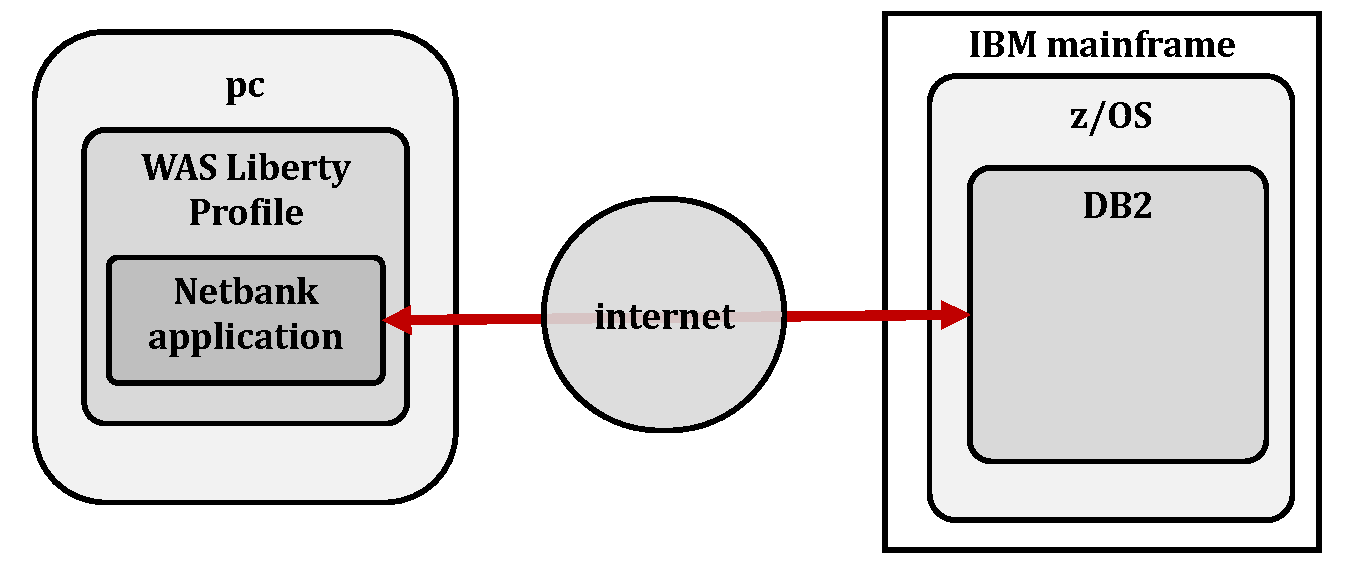
\includegraphics[width = 0.7\textwidth]{figures/communication2.pdf}
\caption{Commucation between modules, when the Netbank application is running on a local server on a PC.}\label{fig:communication_local}
\end{figure}



\begin{figure}[H]
\centering
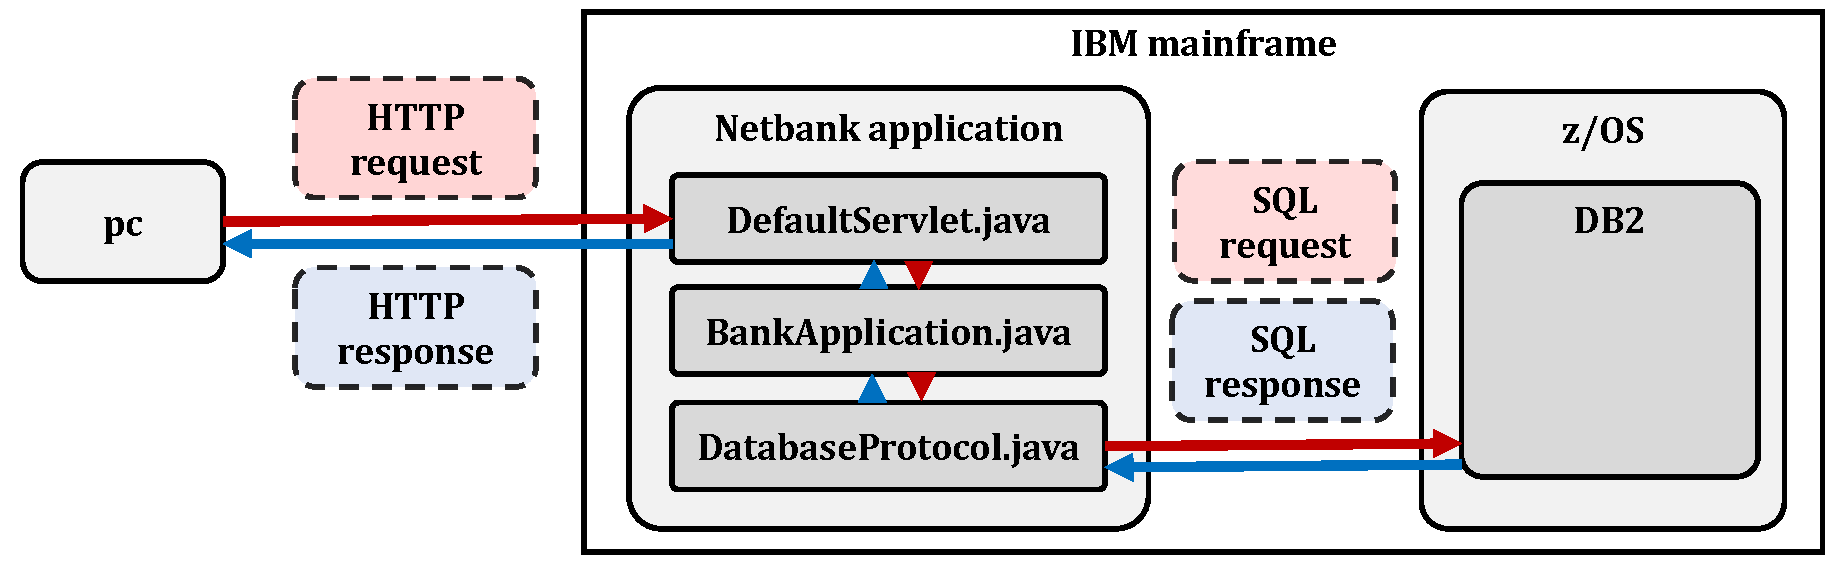
\includegraphics[width = 0.85\textwidth]{figures/interaction_transfer.pdf}
\caption{Commucation between modules when requesting a transfer of money between two accounts. \texttt{DatabaseProtocol} is responsible for interaction with the database.}
\end{figure}


\subsection{Possible extensions (Roar)}

Some ideas when developing the program were not implemented. Ideas which either is common amongst other bank applications, and/or features thought of, as good to have.

\begin{enumerate}
    \item \textbf{Balance plot:} Showing how the balance has changed over a given period as a visual plot. 
    \item \textbf{Account names:} Storing a personal name to each account as well as the generated account ID. Making it more intuitive overview of the accounts for each user.
    \item \textbf{Limited amount of accounts:} An upper limit as to how many accounts a user is allowed to have.
    \item \textbf{Multiple levels of admins:} Allowing for more advanced feature seperation between admins. With the top level admins, able to do all (non illegal) changes to the datastructure. Enabling different levels of authority.
    \item \textbf{Multiple login restriction:} Not allowing a user to be logged in, in multiple computers at the same time. 
    \item \textbf{Account dates:} Creating date stamps for an account when created and deleted.
    \item \textbf{Transfer request:} Making it possible for a user to request a transfer from another user. Similar to the features seen in Mobile Pay.
    \item \textbf{Personal transaction notes:} Giving the user the posibility of storing a personal message with the transfer, not viewable by the reciever of the transfer.
    \item \textbf{Use of scientific notation:} Storing large numbers (greater than $10^7$) in the database without formatting it in scientific notation using doubles.
    \item \textbf{Force lowercase usernames:} When transfering money to a user using the username directly, it should not be possible to send the money to the wrong user, because of an error in character case. 
    \item \textbf{Direct messages:} Making it possible to send messages to a user without a transfer. Possible tech support when messages an admin.
\end{enumerate}





